\chapter{Elastic Stack}
U ovom poglavlju biće opisan Elastik stek, kao primer postojećeg rešenja za prikupljanje i integraciju podataka. Bitno je napomenuti da se dalji tekst oslanja na dokumentaciju trenutno najnovije javno dostupne verzije alata [16], odnosno najnovije verzije komponenti koje čine alat, a koje će biti istaknute pri obrađivanju svake od komponenti. U ovom poglavlju će biti opisani delovi alata neophodni za implementaciju sistema koja će biti data u sledećem poglavlju.

\section{Osnove \textit{Elastic stack}-a}
Elastik stek, takođe poznat kao ELK stek, predstavlja alat, koji postoji kao otvoreno rešenje (eng. open source) kompanije Elastik, a čije funkcionalnosti podrazumevaju: prikupljanje podataka u bilo kom formatu, njihovu obradu, nadogradnju, skladištenje, pretraživanje, analizu i vizuelizaciju u realnom vremenu. Akronim ELK identifikuje ključne komponente ovog steka, a to su: Elasticsearch, Logstash i Kibana [17].

\par
Podaci mogu doći iz bilo kog izvora, što je na slici generalizovano komponentom Beats, koja predstavlja opcioni dodatak ELK steka i služi za slanje operativnih podataka na Logstash. Logstash komponenta predstavlja uređivač (eng. formatter) sistema, njena glavna funkcionalnost jeste prikupljanje ulaznih podataka bilo kog formata, parsiranje podataka i slanje istih u željenom obliku na Elasticsearch. Elasticseach uz pomoć indeksa vrši skladištenje podataka i olakšava njihovo pretraživanje, takozvano pretraživanje celog teksta (eng. full-text search). Tako indeksirani podaci se uz pomoć Kibane mogu vizualno prikazivati i ujedno se vršiti njihova analiza.
Neke od najčešćih vrsta podataka koji se obrađuju uz pomoć ELK steka podrazumevaju: evidentirane (eng. logged), metričke, bezbednosne i podatke biznis logike.

\section{\textit{\textbf{Elasticsearch}}}
\textit{\textbf{Elasticsearch}} je besplatan, distribuirani, otvoreni alat za skladištenje, pretragu i analizu \textit{(eng. search and analytics engine)}, raznih tipova podataka, uključujući tekstualne, numeričke, geo-prostorne \textit{(eng. geospatial)}, strukturne i nestrukturne \cite{elastic-elasticsearch}. Manipulacija podataka je ostvarena \textit{REST API}-jem, a alat omogućava izvanrednu horizontalnu skalabilnost. \textit{\textbf{Elasticsearch}} je zasnovan na \textbf{\textit{Apache Lucene} biblioteci} \cite{apache-lucene}, tj. ideji indeksiranja podataka na osnovu samog sadržaja. Podaci se skladište kao dokumenti, koji pripadaju jednom indeksu, dok je uz pomoć distribuiranog modela, indekse moguće podeliti na manje komponente, odnosno krhotine \textit{(eng. shard)}, koji mogu biti rasprostranjeni kroz veći broj čvorova \textit{(eng. node)}. Trenutno aktuelna verzija na kojoj se zasniva opis alata jeste verzija 8.6.

\subsection{Osnove \textit{\textbf{Elasticsearch}}-a}\label{subsection:osnove-elasticsearch-a}
\textit{\textbf{Elasticsearch}} arhitektura je projektovana za prikupljanje dokumenata, koji se skladište kao \textit{JSON} objekti \cite{json}. Alat podržava ugnježdene strukture, što olakšava obradu kompleksnih podataka i upita. Za praćenje informacija o dokumentima dodeljuju se specijalni atributi, odnosno meta-podaci, koji počinju donjom crtom. Važni meta-podaci su:
\begin{itemize}
    \item \textbf{\_index} – predstavlja kom indeksu dokument pripada. U analogiji, npr. sa relacionim bazama, ovo bi predstavljalo jednu bazu podataka.
    \item \textbf{\_type} – predstavlja klasu, odnosno mapiranje koje bi trebalo da ima svaki dokument koji pripada istom tipu. Ovo je analogno tabeli u relacionim bazama podataka. Trenutna verzija alata ovo polje tretira kao zastarelo \textit{(eng. deprecated)}, ostavljeno je samo radi kompatibilnosti sa starijim verzijama alata.
    \item \textbf{\_id} – jedinstveni identifikator dokumenta u okviru tipa.
    \item \textbf{\_version} – predstavlja broj izmena dokumenta, odnosno koliko puta je dokument bio kreiran, ažuriran, obrisan.
\end{itemize}

\par
Glavni elementi arhitekture \textit{\textbf{Elasticseach}}-a su: \textbf{klaster}, \textbf{čvor}, \textbf{krhotina} i \textbf{analizator}, čija je organizacija predstavljena na slici \ref{diagram:ahritektura-elasticsearch-alata}.

\begin{figure}[H]
    \centering
    \fboxsep=0.025\columnwidth%padding thickness
    \fboxrule=1pt%border thickness
    \fbox{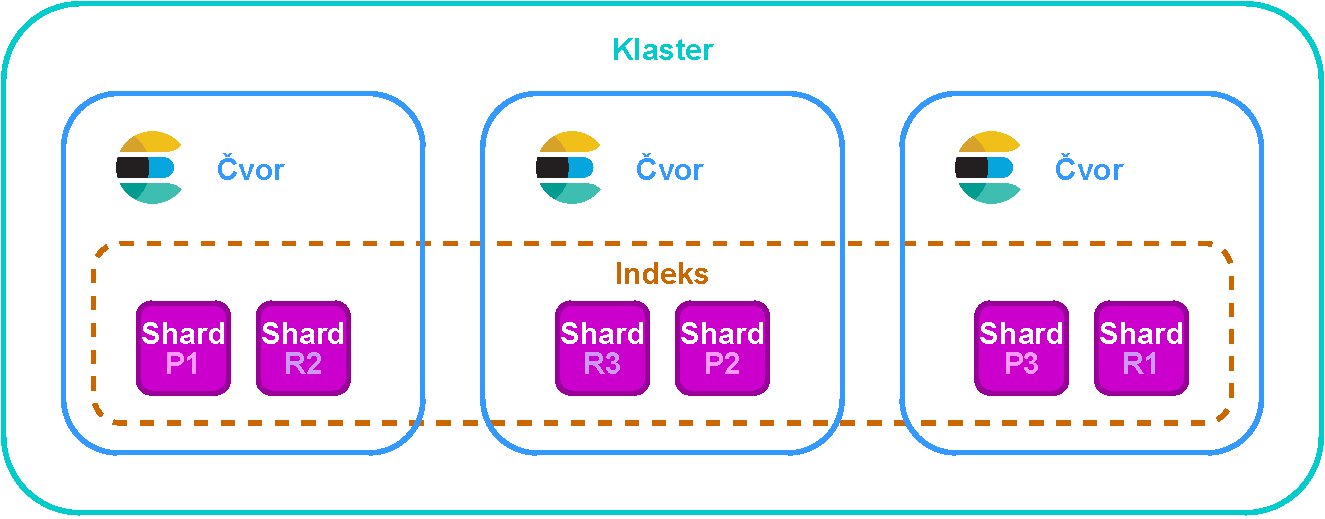
\includegraphics[width=0.95\columnwidth]{images/Elasticsearch-architecture.pdf}}
    \caption{\textit{Arhitektura \textbf{Elasticsearch} alata}}
    \label{diagram:ahritektura-elasticsearch-alata}
\end{figure}

\par
\textbf{Klaster} predstavlja grupu čvorova koji skladište podatke. U okviru konfiguracionog fajla \textit{\textbf{config/Elasticsearch.yml}} \footnote{\textit{YAML} format je dostupan u okviru \cite{YAML}} se može precizirati broj čvorova koji bivaju startovani u klasteru, kao i fizička ili virtualna adresa svakog od čvorova. Čvorovi u okviru jednog klastera su logički povezani i mogu razmenjivati podatke jedni sa drugima. Pri pokretanju, sistem automatski kreira jedan klaster sa jednim čvorom u njemu, što je dovoljno za osnovne potrebe prosečnog korisnika.

\par
\textbf{Čvor} ne predstavlja server, već jednu instancu \textit{\textbf{Elasticsearch}}-a, odnosno proces. Svaka instanca pripada jednom klasteru i zajedno, sa ostalim čvorovima u klasteru radi na rešavanju istog zadatka. Svaki čvor se može konfigurisati tako da obavlja barem jednu, a može obavljati više uloga u klasteru. Uloge koje čvoru mogu biti dodeljene obuhvataju:
\begin{itemize}
\item \textbf{Master čvor} – vrši kontrolu nad klasterom u vidu koordinacije čvorova koji pripadaju klasteru. Ovi čvorovi su odgovorni za operacije nad klasterom \textit{(eng. clasterwide operations)}, poput kreiranja i brisanja indeksa.
\item \textbf{Data čvor} – vrši skladištenje i odgovoran je za invertovani indeks podataka. Ovo je podrazumevana uloga čvora.
\item \textbf{Klijentski čvor} – predstavlja raspoređivač opterećenja \textit{(eng. load balancer)}\cite{Sanders2019-hv} koji vrši usmeravanje pristiglih zahteva različitim čvorovima u klasteru.
\end{itemize}

\par
Za ostvarivanje komunikacije se koriste dva glavna porta:
\begin{itemize}
    \item \textbf{Port 9200} – koristi se za filtriranje zahteva koji dolaze izvan klastera. Ovo su zahtevi \textit{REST API}-ja koji se koriste za izvršavanje upita, indeksiranje i slično.
    \item \textbf{Port 9300} – koristi se za među-čvornu \textit{(eng. inter-node)} komunikaciju.
\end{itemize}

\par
\textbf{Krhotina} predstavlja podskup dokumenata u okviru jednog indeksa. Naime, indeks nema ograničen broj dokumenata, niti ograničen memorijski kapacitet koji može da skladišti. Ukoliko se desi prekoračenje memorije na jednom od čvorova, \textit{\textbf{Elasticsearch}} prestaje sa radom i javlja grešku. Kako bi se ovaj problem rešio, indeksi se dele na krhotine, koje označavaju skalabilnu jedinicu za indeksiranje i omogućavaju distribuciju jednog indeksa na više čvorova. Ovim se postiže horizontalna skalabilnost sistema. Svaka krhotina funkcioniše kao nezavisan \textit{Lucene} indeks \cite{apache-lucene}, koji može biti skladišten bilo gde u klasteru.

\par
\textbf{Replika} predstavlja kopiju krhotine indeksa, dok se originalna krhotina naziva primarnom \textit{(eng. primary shard)}. Redundantnost podataka je glavni mehanizam na koji se sistemi otporni na greške oslanjaju \cite{Sanders2019-hv}. S obzirom da se radi o distribuiranom sistemom, ukoliko bi neki od čvorova otkazao, krhotine indeksa koje sadrži bi bile nedostupne, a samim tim i svi dokumenti koji se nalaze u nedostupnim podskupovima. Iz tog razloga se formiraju replike i dodeljuju različitim čvorovima u sistemu. Pored otpornosti na otkaze, ovo omogućava i brže pretraživanje podataka, jer više čvorova koji sadrže istu kopiju krhotine indeksa mogu istovremeno da vrše njenu pretragu i time ubrzaju proces pretrage indeksa u celini. Broj replika nije ograničen i mogu se precizirati nakon kreiranja indeksa, međutim, treba voditi računa jer iako je ovim čitanje ubrzano, svaka modifikacija je time znatno složenija.

\par
\textbf{Analizatori} imaju zadatak da vrše parsiranje fraza i izraza u konzistentne termine. Ovo se odvija u procesu indeksiranja. Svaki analizator je sačinjen od jednog tokenizatora \textit{(eng. tokenizer)} \footnote{Tokenizacija je proces razgraničenja i moguće klasifikacije delova niza ulaznih znakova. Dobijeni tokeni se zatim prosleđuju nekom drugom obliku obrade. Proces se može smatrati podzadatkom raščlanjivanja ulaza.\cite{tokenization}} i većeg broja filtera tokena. Kada se naiđe na određeni izraz, tokenizator može da podeli izraz u prethodno definisane termine. U ovome se krije još jedna tajna brze pretrage podataka.

\section{\textit{\textbf{Logstash}}}
\textit{\textbf{Logstash}} je alat otvorenog koda za prikupljanje podataka sa mogućnostima nadovezivanja \textit{(eng. pipelining)} u realnom vremenu. Alat može dinamičnim putem objediniti podatke iz različitih izvora, obogatiti ih, normalizovati i na kraju dostaviti podatke na unapred definisana odredišta. Ovim se pruža mogućnost prečišćavanja podataka za različite slučajeve upotrebe, naprednu analizu ili vizuelizaciju \cite{elastic-logstash}.

\par
Na početku je \textit{\textbf{Logstash}} bio korišćen za prikupljanje podataka evidencije \textit{(eng. log)}, međutim, mogućnosti koje pruža su prevazišle taj slučaj korišćenja. Naime, bilo koja vrsta događaja može biti prosleđena alatu, uz pomoć širokog spektra ulaznih dodataka \textit{(eng. input plugins)}, primljeni događaji mogu biti integrisani i transformisani uz pomoć dodataka za filtriranje \textit{(eng. filter plugins)} i na kraju tako formatirani podaci mogu biti prosleđeni na razne vrste izlaza, uz pomoć izlazih dodataka \textit{(eng. output plugins)}. Sam proces obrade je podržan velikim brojem često korišćenih kodera, a pritom je alat dizajniran za obradu velike količine podataka u realnom vremenu. Alat je razvijen u programskom jeziku JRuby i izvršava se na javinoj virtuelnoj mašini \textit{(eng. Java Virtual Machine)}, skraćeno \textit{JVM} \cite{jvm}.

\subsection{Kako \textit{\textbf{Logstash}} funkcioniše?}
\textit{\textbf{Logstash}} za sebe ima vezane cevovode, ili tokove podataka \textit{(eng. pipeline)} definisane ulaznim, transformacionim i izlaznim etapama. Ulazi očitavaju događaje, filteri ih modifikuju, a izlazi tako modifikovane događaje dostavljaju na definisana odredišta. Ulazi i izlazi imaju unapred podržane kodeke \footnote{Kodek \textit{(eng. codec)} kompresuje ili dekompresuje bilo koji sadržaj u i iz bajtova.\cite{codec}}, koji omogućavaju kodiranje i dekodiranje podataka pri ulazu i izlazu iz toka obrade, bez korišćenja transformacionih filtera. Primer jednog toka podataka prikazan je na slici \ref{diagram:primer-logstash-toka-podataka}.

\begin{figure}[H]
    \centering
    \fboxsep=0.025\columnwidth%padding thickness
    \fboxrule=1pt%border thickness
    \fbox{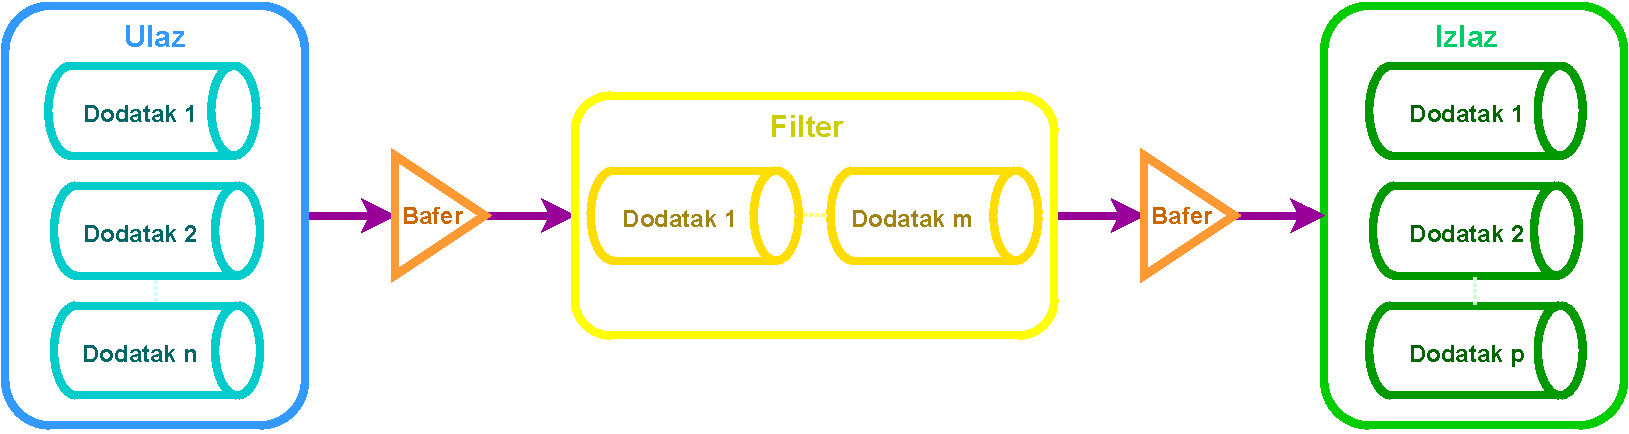
\includegraphics[width=0.95\columnwidth]{images/Logstash-pipeline.pdf}}
    \caption{\textit{Primer \textbf{Logstash} toka podataka}}
    \label{diagram:primer-logstash-toka-podataka}
\end{figure}

\par
Svaki dodatak koji se koristi u okviru ulazne etape se izvršava u sopstvenoj niti i svaki od njih upisuje događaje u centralizovani red čekanja koji je ili u radnoj memoriji pokrenutog procesa, ili može biti na disku. Svaki radnik toka podataka \textit{(eng. pipeline worker)} uzima blok događaja iz reda čekanja, sprovodi blok kroz definisane dodatke u okviru filter etape i na kraju šalje obrađene događaje na svaki od definisanih dodataka izlazne etape. Veličina bloka, kao i broj radnika toka podataka, odnosno niti, je podesiv kroz konfiguracione fajlove \textit{\textbf{Logstash}}-a.

\par
\textit{\textbf{Logstash}} podrazumevano koristi redove čekanja koji se nalaze u radnoj memoriji za baferovanje događaja između etapa, ulaz i filter etapa, odnosno filter i izlaz etapa, što je brže rešenje. Međutim pri nastanku greške, odnosno obustavi procesa, baferovani podaci bivaju izgubljeni.

\par
\textbf{Ulaznim dodacima} se definiše izvor podataka koji ulaze u sistem. Najčešće korišćeni ulazni dodaci podrazumevaju:
\begin{itemize}
\item \textbf{file} – vrši čitanje fajla sa fajl sistema nalik \textit{Unix} komandi \mintinline{shell-session}{tail -0F},
\item \textbf{syslog} – osluškuje na podrazumevanom portu 514, koji predstavlja port za \textit{syslog} poruke u \textit{Unix}-u i parsira ih na osnovu RFC3164 formata \cite{syslog-protocol},
\item \textbf{redis} – vrši čitanje sa \textit{Redis} servera, konkretno sa \textit{Redis} kanala i listi. \textit{Redis} \cite{redis} je često korišćen kao berzijanac poruka \textit{(eng. message broker)} u centralizovanoj instalaciji \textit{\textbf{Logstash}}-a i služi za skladištenje događaja u okviru reda čekanja,
\item \textbf{beats} – vrši obradu podataka koji se dobijaju uz pomoć \textit{Beats} alata \cite{elastic-beats}.
\end{itemize}

\par
textbf{Filter dodaci} predstavljaju procesne uređaje koji posreduju tokom podataka. Filteri mogu biti kombinovani uslovima koji diriguju da li se određena faza obrade izvršava ili ne, u zavisnosti od kriterijuma koji se ispituje. Najčešće korišćeni dodaci za filtriranje su:
\begin{itemize}
\item \textbf{grok} – parsira i gradi proizvoljan tekst. Ovaj dodatak je trenutno najpogodnije rešenje za parsiranje nestrukturnih tokova podataka u podatke koji imaju strukturu i moguće je nad njima izvršavati upite,
\item \textbf{mutate} – izvršava generalne transformacije nad poljima događaja, poput: preimenovanja, uklanjanja, zamene, modifikacije i slično,
\item \textbf{drop} – izvršava obustavu događaja u potpunosti. Korisno pri događajima koji imaju debug nivo ozbiljnosti,
\item \textbf{clone} – vrši replikaciju događaja, sa mogućnošću za dalje dodavanje i uklanjanje pojedinih polja,
\item \textbf{geoip} – nadograđuje \textit{IP} adresu geo-prostornim koordinatama, kao i dostupnim informacijama za iste.
\end{itemize}

\par
\textbf{Izlazni dodaci} predstavljaju destinacije konačne etape u izvršavanju toka podataka \textit{\textbf{Logstash}}-a. Događaj može proći kroz više izlaza, međutim, njegova obrada je završena kada prođe kroz sve navedene izlaze. Najčešće korišćeni dodaci za izlaz podrazumevaju:
\begin{itemize}
    \item \textbf{elasticsearch} – šalje događaj na \textit{Elasticsearch}, samim tim se vrši indeksiranje podataka koji dalje mogu lako da se pretražuju i vizualizuju u \textit{Kibani}.
    \item \textbf{stdout} – ispisuje događaj na standardni izlaz.
    \item \textbf{file} – skladišti formatiran događaj na fajl u fajl sistemu.
    \item \textbf{graphite} – šalje događaj na  \textit{graphite}, koji predstavlja popularan alat otvorenog koda za skladištenje podataka metrike. \cite{graphite}
    \item \textbf{statsd} – šalje podatke na  \textit{statsd}. Ovo je pozadinski servis  \textit{(eng. deamon)}, koji se izvršava na  \textit{Node.js} platformi, a čija je funkcija osluškivanje podataka statistike poslate  \textit{UDP} transportnim protokolom i prosleđivanje primljenih podataka na jedan ili više priključivih  \textit{(eng. pluggable)} pozadinskih  \textit{(eng. backend)} servisa, poput gore navedenog  \textit{graphite} servisa. \cite{statsd}
\end{itemize}

\subsection{\textit{\textbf{Logstash}} konfiguracioni fajlovi}
\textit{\textbf{Logstash}} sadrži dve vrste konfiguracionih fajlova, a to su:
\begin{itemize}
    \item \textbf{Pipeline konfiguracioni fajlovi}, koji definišu sam tok podataka. Izgled ovih fajlova će biti detaljnije objašnjen u nastavku.
    \item \textbf{Settings konfiguracioni fajlovi}, koji definišu inicijalizaciju i tok rada samog \textit{\textbf{Logstash}} procesa. Ovi fajlovi su generisani pri instaliranju samog \textit{\textbf{Logstash}} servisa i podrazumevaju fajlove:
    \begin{itemize}
        \item[o] \textbf{Logstash.yml} – sadrži konfiguracione indikatore \textit{(eng. flags)} za instancu programa. Ovde se mogu definisati: tip i lokacija bafera koji se koristi za red čekanja između etapa, veličina bloka događaja koju obrađuje jedan radnik, nivo evidentiranja \textit{(eng. logging level)} i mnoga druga podešavanja.
        \item[o] \textbf{Pipelines.yml} – sadrži konfiguraciju većeg broja tokova podataka koji će se izvršavati u okviru jedne instance \textit{\textbf{Logstash}}-a. Ovde se između ostalog navodi putanja do same konfiguracije toka podataka, kao i broj radnika u okviru toka, identifikator toka i slično.
        \item[o] \textbf{Jvm.options} – sadrži podešavanja za \textit{JVM} indikatore. Ovde se između ostalog može definisati minimalna i maksimalna veličina radne memorije dodeljene procesu.
        \item[o] \textbf{Log4j2.properties} – sadrži podrazumevana podešavanja za \textit{log4j} biblioteku \cite{log4j}.
    \end{itemize}
\end{itemize}

\subsubsection{Struktura konfiguracionih fajlova}
\textit{\textbf{Logstash}} konfiguracioni fajlovi za tokove podataka su pisani u specijalnom jeziku \cite{logstash-pipeline-language} koji je razvijen od strane samih osnivača programa. Jezik podseća na \textit{JSON} format sa par izuzetaka, ali je vrlo jednostavan za razumevanje.
Tok podataka, \textit{pipeline} ima odvojene segmente za ulaznu, filter i izlaznu etapu, čija je oblast važenja uokvirena vitičastim zagradama. U okviru svake od etapa se mogu navesti dodaci koji se koriste.  Bitno je naglasiti da se dodaci u okviru ulazne etape izvršavaju konkurentno, dok se u filter i izlaznoj etapi izvršavaju sekvencijalno.

\par
Primer jednog konfiguracionog fajla je dat u okviru slike \ref{code:primer-konfiguracije-toka-podataka}.
\begin{listing}[H]
\begin{minted}[frame=single,
               framesep=3mm,
               linenos=true,
               xleftmargin=21pt,
               tabsize=4]{js}
input {
    http {
        port => 3333
        tags => gateway
    }
}
filter {
    . . . 
}
output {
    . . .
}
\end{minted}
\caption{\textit{Primer konfiguracije toka podataka}}
\label{code:primer-konfiguracije-toka-podataka}
\end{listing}

\par
Dodaci mogu zahtevati vrednosti za određena podešavanja. Tipovi vrednosti koje postoje u okviru konfiguracije su:
\begin{itemize}
    \item \textbf{Lista} – definiše se uglastim zagradama, dok su elementi unutar zagrada odvojeni zarezima,
    \item \textbf{Logička vrednost} – definiše se vrednostima \mintinline{js}{true} i \mintinline{js}{false},
    \item \textbf{Bajt} – definiše se kao string koji sadrži broj bajtova sa mernom jedinicom, bilo da je u pitanju SI (osnova 1000), ili binarna (osnova 1024) merna jedinica. Polje nije osetljivo na velika slova \textit{(eng. case-insensitive)} i prepoznaje razmak između vrednosti i jedinice. Ukoliko se ne napiše jedinica, već samo celobrojna vrednost, podrazumeva se da vrednost predstavlja egzaktan broj bajtova,
    \item \textbf{Kodek} – definiše ime jednog od \textit{\textbf{Logstash}} kodeka, koji se može naznačiti i u ulaznim i u izlaznim etapama. Kada se nađe u ulaznoj etapi, predstavlja način dekodiranja podataka koji ulaze u tok, dok na izlazu predstavljaju način kodiranja u određeni format,
    \item \textbf{Heš mapa} – definiše kolekciju ključ-vrednost elemenata u formatu \textit{"polje" => "vrednost"}, gde se elementi razdvajaju blanko znacima, ne zapetama kao kod listi i nizova,
    \item \textbf{Broj} – obuhvata realne brojeve, odnosno \textit{integer} i \textit{float} vrednosti,
    \item \textbf{Lozinka} – string vrednost koja ne biva evidentirana,
    \item \textbf{URI} – string vrednost koja predstavlja identifikator resursa, može biti potpun ili parcijalni \textit{URL}. Ukoliko sadrži korisničko ime i lozinku, takođe se neće evidentirati,
    \item \textbf{Putanja} – definiše validnu putanju do resursa na sistemu,
    \item \textbf{String} – sekvenca karaktera, ukoliko sadrži blanko znake, neophodno je ograditi ga jednostrukim ili dvostrukim znakom navoda,
    \item \textbf{Referenca na polje} – predstavlja putanju do polja u događaju, ukoliko se radi o polju koje je u korenu događaja, onda se može koristiti notacija \mintinline{js}{[polje]} ili se izostaviti uglaste zagrade, polje. Ukoliko se referencira ugnježdeno polje, onda je neophodno koristiti notaciju sa uglastim zagradama i to po ugledu na oblik \mintinline{js}{[polje prvog nivoa][polje drugog nivoa]...[polje n-tog nivoa]}.
    \item \textbf{Komentari} se označavaju kao u programskim jezicima \textit{Perl}, \textit{Ruby} i \textit{Python}, odnosno počinju znakom taraba (\#).
\end{itemize}

\par
\textbf{Uslovne strukture} \textit{(eng. conditionals)} su podržane, imaju poznatu strukturu kao i u ostalim programskim jezicima \mintinline{python}{if, else if, else}, a koriste se za dodatno kontrolisanje filter i izlazne etape toka podataka. Primer strukture je dat u nastavku \ref{code:uslovne-strukture-u-konfiguracionom-fajlu-toka-podataka}.
\begin{listing}[H]
\begin{minted}[frame=single,
               framesep=3mm,
               linenos=true,
               xleftmargin=21pt,
               tabsize=4]{python}
if EXPRESSION {
    ...
} else if EXPRESSION {
    ...
} else {
    ...
}
\end{minted}
\caption{\textit{Uslovne strukture u konfiguracionom fajlu toka podataka}}
\label{code:uslovne-strukture-u-konfiguracionom-fajlu-toka-podataka}
\end{listing}

\par
\textbf{Izraz} \textit{(eng. expression)} predstavlja logički izraz koji se svodi na jednu od logičkih vrednosti \mintinline{js}{true}, ili \mintinline{js}{false}. Ukoliko izraz sadrži referencu na polje, vrednost izraza će biti \mintinline{js}{false} ukoliko: polje ne postoji, polje ima nedefinisanu vrednost \mintinline{js}{null} ili postoji i ima vrednost \mintinline{js}{false}. Podržani operatori u okviru jezika podrazumevaju:
\begin{itemize}
\item Operatore poređenja:
\begin{itemize}
\item[o] Jednakost: \textbf{==}, \textbf{!=}, \textbf{<}, \textbf{>}, \textbf{<=}, \textbf{>=}
\item[o] Regularni izraz: \textbf{=~}, \textbf{!~}
\item[o] Provera sadržaja: \textbf{in}, \textbf{not in}
\end{itemize}
\item Logičke operatore: \textbf{and}, \textbf{or}, \textbf{nand}, \textbf{xor}
\item Unarni operator: \textbf{!}
\end{itemize}

\par
Konkretan primer uslovne strukture sa izrazima je dat na slici \ref{code:primer-izraza-u-okviru-uslovnih-struktura}.
\begin{listing}[H]
\begin{minted}[frame=single,
               framesep=3mm,
               linenos=true,
               xleftmargin=21pt,
               tabsize=4,
               fontsize={\fontsize{10}{10}\selectfont}]{python}
filter {
    if [fooVal] in ["test", "debug"] and ([logLevel] != "debug") {
        mutate { add_tag => "testing" }
    }
    if [foo] =~ "[0-9]+" {
        mutate { add_tag => "contains numbers" }
    }
    if "%{+HH}" < "16" {
      mutate { add_tag => "Before 16h" }
    }    
}
output {
    if "testing" not in [tags] {
        elasticsearch{
            ...
        }
    }
}
\end{minted}
\caption{\textit{Primer izraza u okviru uslovnih struktura}}
\label{code:primer-izraza-u-okviru-uslovnih-struktura}
\end{listing}

\par
Svakom događaju koji se generiše u ulaznoj etapi obrade se pridružuju polja koja bliže opisuju događaj. Ova polja su rezervisana, njihov tip zavisi od implementacije samog ulaznog dodatka koji ih generiše, a namenjeni su boljoj kontroli toka obrade:
\begin{itemize}
    \item \textbf{@metadata} – heš mapa namenjena za skladištenje pomoćnih podataka u toku obrade. Ovo polje je dostupno u filter i izlaznoj etapi, međutim, podrazumevano se ne šalje na izlazne dodatke.
    \item \textbf{@timestamp} – predstavlja vremenski trenutak u kom je generisan događaj. Iz ovog polja se čitaju podaci koje koristi \textit{sprintf} format, koji omogućava referenciranje vrednosti iz ostalih polja događaja.
    \item \textbf{@version} – predstavlja verziju dodatka koji je generisao događaj.
    \item \textbf{tags} – niz vrednosti koji se koriste radi bližeg opisivanja događaja.
\end{itemize}

\subsection{Dodaci toka obrade}
\textbf{Dodaci toka obrade} \textit{(eng. pipeline plugins)} su programi napisani u programskom jeziku \textit{Java} ili \textit{Ruby}, koji predstavljaju alat za olakšavanje kontrole samog toka obrade, od ulaza, preko obrade, do izlaza samih podataka. Ove programe može napisati bilo ko u programskom jeziku \textit{Java} ili \textit{Ruby} i publikovati ih na javni \textit{Github} repozitorijum sa kog ostali korisnici mogu da ih povlače i koriste u svojim sistemima. Samim tim, \textit{\textbf{Logstash}} ima jako veliki skup dodataka koji mogu biti korišćeni, dok će ovaj rad nadalje obraditi samo one koji su neophodni za razumevanje sistema koji se implementira.

\par
\textbf{TCP ulazni dodatak} \cite{tcp-plugin} vrši čitanje poruka poslatih preko mreže, tako što osluškuje poruke TCP protokola, generišući odgovarajuće događaje za tok podataka u kom je konfigurisan. 

\par
\textbf{Grok filter dodatak} \cite{grok-plugin} vrši parsiranje proizvoljnog teksta i njegovo prevođenje u strukturni podatak, nad kojim se mogu pisati upiti. Funkcioniše tako što koristi regularne izraze za pronalaženje šablona u okviru tekstualnih polja. Sintaksa koju prati ovaj dodatak je \textbf{\%{SINTAKSA:SEMANTIKA}}. Sintaksa predstavlja ime unapred definisanog šablona regularnog izraza koji se koristi za identifikovanje dela teksta, dok semantika predstavlja identifikator pronađenog teksta koji se dalje može koristiti u toku podataka. Pored unapred definisanih šablona, mogu se direktno pisati regularni izrazi za pronalaženje šablona. Sintaksa regularnih izraza koja se koristi je \textit{Onigurama} \cite{onigurama}, koja ima izgled \textit{(?<identifikator polja>šablon)}. Još jedan način jeste kreiranje sopstvenih šablona u odvojenim fajlovima (putanje do fajlova se definišu u konfiguraciji dodatka), dok novo-definisani šablon ima izgled \textit{IME\_ŠABLONA ŠABLON}.

\par
\textbf{Mutate filter dodatak} \cite{mutate-plugin} omogućava generalizaciju mutacija nad poljima događaja. Moguće su operacije: preimenovanja, zamene, modifikacije polja u okviru događaja i slično. Redosled operacija u okviru dodatka je unapred ustanovljen, odnosno ne prati redosled navođenja operacija u okviru konfiguracije. Ukoliko je neophodno izvršiti više operacija koje ne prate ovakav redosled, neophodno je definisati više \textit{mutate} filter dodataka u odgovarajućem redosledu. 

\par
\textbf{Geoip filter dodatak} \cite{geoip-plugin} nadograđuje događaje informacijama o geo-prostornoj lokaciji prosleđene \textit{IP} adrese. Ovaj dodatak je zasnovan na podacima iz \textit{MaxMind GeoLite2} baze podataka \cite{maxmind-geolite}, koja dolazi kao podrazumevana baza dodatka. Moguće je kroz opcije konfigurisati bazu podataka, odnosno promeniti podrazumevanu. Primer odgovora koji se dobija za prosleđenu \textit{IP} adresu dat je u okviru slike \ref{code:primer-podataka-koje-pruza-geoip-filter-dodatak-za-prosledjenu-ip-adresu}.

\begin{listing}[H]
\begin{minted}[frame=single,
               framesep=3mm,
               linenos=true,
               xleftmargin=21pt,
               tabsize=4]{js}
{
    "ip": "12.34.56.78",
    "geo": {
        "city_name": "Seattle",
        "country_name": "United States",
        "cotinent_code": "NA",
        "continent_name": "North America",
        "country_iso_code": "US",
        "postal_code": 98106,
        "region_name": "Washington",
        "region_code": "WA",
        "region_iso_code": "US-WA",
        "timezone": "America/Los_Angeles",
        "location": {
            "lat": 47.6062,
            "lon": -122.3321,
        }
    },
    "domain": "example.com",
    "asn": {
        "number": 98765,
        "organization": {
            "name": "Elastic, NV"
        }
    },
    "mmdb": {
        "isp": "InterLi Supra LLC",
        "dma_code": 819,
        "organization": "Elastic, NV"
    }
}
\end{minted}
\caption{\textit{Primer podataka koje pruža geoip filter dodatak za prosleđenu IP adresu}}
\label{code:primer-podataka-koje-pruza-geoip-filter-dodatak-za-prosledjenu-ip-adresu}
\end{listing}

\par
\textbf{Http filter dodatak} \cite{http-plugin} omogućava integraciju sa eksternim \textit{Web} servisima ili \textit{REST API}-jima, tako što osposobljava \textit{\textbf{Logstash}} da šalje zahteve podesive strukture na odgovarajuće krajnje tačke \textit{(eng. endpoint)}, kako bi obogatio događaj koji se obrađuje dodatnim informacijama. Parametar koji definiše zaglavlja zahteva \textit{(eng. headers)} koji se šalju bivaju definisana u okviru \textbf{@metadata} polja, kako ne bi okupirali destinacije na izlazu. Ovo je vrlo podesiv dodatak i ima veliki broj opcija za konfiguraciju.

\par
\textbf{Dns filter dodatak} \cite{dns-plugin} pruža pretragu stavki, kanoničkih imena \textit{(eng. CNAME)}, ili stavki adresa \textit{(eng. A record)}, odnosno ukoliko je u pitanju inverzni \textit{DNS}, pretražuju se pointer stavke \textit{(eng. pointer record, PTR)}. Bitno je napomenuti da ovaj dodatak može da obradi samo jednu stavku, dakle za veći broj stavki je potrebno više puta iskoristiti ovaj dodatak, s tim što ovakvo podešavanje može drastično da uspori sistem. 

\par
\textbf{Elasticseach izlazni dodatak} \cite{elasticsearch-plugin} omogućava skladištenje vremenskih serija podataka, poput podataka evidencije, događaja i metrike, kao i podataka čije skladištenje nije bazirano na vremenskim intervalima, direktno u \textit{Elasticsearch}. S obzirom da se radi o dodatku koji radi sa osnovnim proizvodom kompanije, ovaj dodatak je jako fleksibilan i može kontrolisati razne segmente vezane za operacije u \textit{Elasticsearch}-u. Najbitnije opcije u okviru dodatka, koje se vezuju za temu ovog rada podrazumevaju:
\begin{itemize}
    \item \textbf{action} – enumeracija(\textit{index, delete, create, update}) koja definiše koja vrsta operacije biva izvršavana. Podrazumevana vrednost za vremenske serije podataka, odnosno tokove podataka je \textit{create}, dok je \textit{index} podrazumevana vrednost za podatke koji se ne vezuju za vremenske intervale.
    \item \textbf{index} – string koji predstavlja indeks u koji se upisuju podaci obrađeni u okviru toka podataka
    \item \textbf{hosts} – uri tip vrednosti, koji predstavlja jednu ili više adresa čvorova na kojima je pokrenuta instanca \textit{Elasticsearch}-a. Podrazumevana vrednost je \mintinline{python}{[//127.0.0.1]}.
\end{itemize}
\section{\textit{\textbf{Kibana}}}
\textit{\textbf{Kibana}} je aplikacija otvorenog koda koja pruža pregledan korisnički interfejs ka \textit{Elastic stack}-u, uz mogućnosti pretraživanja, vizuelizacije i analize podataka indeksiranih \textit{Elasticsearch}-om. Takođe poznata i kao alat za kreiranje raznovrsnih grafikona \textit{(eng. charts)}, \textit{\textbf{Kibana}} omogućava nadgledanje, upravljanje i održavanje bezbednosti klastera u \textit{Elastic stack}-u. Prvi put je postala dostupna javnosti 2013. godine, dok je trenutna aktuelna verzija 8.6, na osnovu koje će biti opisani pojedini detalji same aplikacije \cite{elastic-kibana}.

\par
Glavna primena \textit{\textbf{Kibana}}-e podrazumeva: pretraživanje, vizualizaciju indeksiranih podataka u okviru \textit{Elasticsearch}-a, kao i analizu podataka kroz kreiranje grafikona, poput: poluga, pita, tabela, histograma i mapa. Komandna tabla \textit{(eng. dashboard)} kombinuje ove elemente na jedan pano i time omogućava analitički pregled podataka u realnom vremenu za razne slučajeve korišćenja, poput:
\begin{enumerate}
    \item analize podataka evidencije, 
    \item nadgledanja metričkih podataka infrastrukture i kontejnera, 
    \item vizuelizaciju geo-prostornih podataka, 
    \item analizu sigurnosnih podataka, 
    \item analizu podataka biznis logike.
\end{enumerate}

\subsection{Upitni jezik \textit{\textbf{Kibana}}-e}
\textit{\textbf{Kibana}} koristi specifični upitni jezik nazvan \textit{\textbf{Kibana Query Language}} \cite{kql}, ili skraćeno \textit{\textbf{KQL}}, kojim je omogućeno jednostavno filtriranje podataka u svrhu vizualizacije. Ovaj jezik se razlikuje od standardnog \textit{Lucene }upitnog jezika, jer ne omogućava pretragu uz pomoć regularnih izraza ili takozvanu pomućenu \textit{(eng. fuzzy)} pretragu podataka, međutim omogućena je pretraga ugnježdenih polja kao i takozvanih skriptovanih polja \textit{(eng. scripted fields)}.

\par
U okviru jezika se mogu identifikovati podvrste upitnog jezika: \textbf{upiti termina}, \textbf{upiti Bulove algebre}, \textbf{opsežni upiti}, \textbf{upiti koji koriste džokere} i \textbf{upiti nad ugnježdenim poljima}.

\par
\textbf{Upiti termina} \textit{(eng. terms query)}, koji koriste egzaktan stil pretrage. Sintaksa ovog upita ima oblik \textit{<putanja do polja> : <list termina>}, gde putanja do polja predstavlja ugnježdena polja počevši od korena dokumenta, sve do polja koje se pretražuje, nivoi su razdvojeni tačkom. Lista termina predstavlja prihvatljive vrednosti u okviru navedenog polja, dok se različiti termini odvajaju razmakom, a ukoliko se pretražuju egzaktne fraze, koriste se znaci navođenja. Putanja do polja i lista termina se odvajaju specijalnim karakterom dvotačka, na koji može da se gleda kao na operator \textit{in}.

\par
\textbf{Upiti Bulove algebre} \textit{(eng. boolean queries)} predstavljaju kombinovanje prethodno navedene podvrste upita logičkim operatorima: \textbf{or}, \textbf{and} i \textbf{not}. Po pravilu, \textbf{and} ima viši prioritet od operatora \textbf{or}, ukoliko je neophodna drugačija logika, koriste se zagrade.

\par
\textbf{Opsežni upiti} \textit{(eng. range queries)} predstavljaju upite koji numeričke i vrednosti datuma navedenih polja porede operatorima jednakosti: \textbf{>}, \textbf{>=}, \textbf{<} i \textbf{<=}. Moguće je koristiti i matematičke izraze pri poređenju vrednosti, što je jako pogodno za datume.

\par
\textbf{Upiti koji koriste džokere} \textit{(eng. wildcard)}, koji je označen znakom \textbf{*} i može biti ili u delu putanje polja, čime se pokriva veći broj polja, ili u okviru vrednosti koje se traže u poljima i time pokriva veći spektar vrednosti, jer menja odgovarajući deo bilo kojom sekvencom bilo koje dužine.

\par
\textbf{Upiti nad ugnježdenim poljima} \textit{(eng. nested field queries)} omogućavaju dva pristupa u filtriranju ugnježdenih dokumenata:
\begin{itemize}
    \item Filtriranje jednog dokumenta na osnovu određenih delova upita\\
\textit{<polje>:\{ <ugnježdeno polje 1>:<izraz 1> and <ugnježdeno polje 2>:<izraz 2> \}}
    \item Filtriranje više dokumenata na osnovu određenih delova upita \\
\textit{<polje>:\{ <ugnježdeno polje 1>:<izraz 1> \} and <polje>:\{ <ugnježdeno polje 2>:<izraz 2> }\}
\end{itemize}